%---------------------------------------------------------------------------%
%->> Chapter 5: 实验验证与分析
%---------------------------------------------------------------------------%

\chapter{实验验证与分析}

本章围绕故障指纹检索、SOP 自动化构建、端到端根因定位和消融实验四个方面，对本文方法进行实验验证与分析。首先介绍研究问题、实验环境、数据集和评估指标，随后分别给出实验结果并进行分析，最后对本章内容作总结。

% 第5章表格统一样式
\newcommand{\ChapFiveTableHeadColor}{gray!15}
\newcommand{\ChapFiveTableStatColor}{gray!10}
\newcommand{\ChapFiveTableSetup}{%
    \renewcommand{\arraystretch}{1.3}%
    \small%
    \setlength{\tabcolsep}{4.5pt}%
}
\newcommand{\ChapFiveTableNote}[1]{%
    \vspace{0.4em}
    \small\textbf{注：}#1%
}

%---------------------------------------------------------------------------%
%->> 实验目的
%---------------------------------------------------------------------------%

\section{实验目的}

本章主要回答以下四个研究问题。

\textbf{RQ1：PMF 能否为相似故障检索提供稳定且具有区分性的表示。}
这一问题聚焦于传播感知多模态故障指纹构建方法的有效性，重点考察历史故障在统一表示空间中能否形成较好的类内聚集，并在“故障组件角色 + 故障类型”的粒度上实现稳定检索。

\textbf{RQ2：SOP 自动化构建方法能否生成可执行、可复用的 SOP，并用于未见故障的诊断。}
这一问题关注离线阶段自动构建的 SOP 是否会随着迭代逐步完善，以及这些 SOP 能否迁移到测试集中的未见故障实例上，支撑实际诊断过程。

\textbf{RQ3：与传统基线方法和大语言模型基线方法相比，本文方法在端到端根因定位任务中的表现如何。}
这一问题主要比较不同方法在真实故障场景中的排序质量，重点考察 Top-K 命中情况以及首个正确结果所在的位置。

\textbf{RQ4：SOP 引导、逃逸机制以及焦点与感知域约束分别对端到端定位性能有何影响。}
为回答这一问题，本文通过消融实验分别移除上述三类机制，观察性能变化，并分析各组件具体作用。

%---------------------------------------------------------------------------%
%->> 5.2 实验设置
%---------------------------------------------------------------------------%

\section{实验设置}

本节介绍实验环境、数据集和评估指标，后续实验均基于这些设置展开。

\textbf{实验环境}：实验平台配置见表\ref{tab:experiment_config}。

\begin{table}[htbp]
    \centering
    \bicaption{\enspace 实验环境配置}{\enspace Experimental Environment Configuration}
    \label{tab:experiment_config}
    \ChapFiveTableSetup
    \begin{tabular}{ll}
        \toprule
        \rowcolor{\ChapFiveTableHeadColor}
        \textbf{名称} & \textbf{配置信息} \\
        \midrule
        操作系统 & Ubuntu 24.04.4 LTS (Noble Numbat) \\
        内核版本 & Linux 6.8.0-100-generic \\
        CPU & Intel Xeon Platinum 8368 @ 2.40GHz (152 vCPUs) \\
        内存 & 504 GB \\
        磁盘 & 438 GB SSD (系统盘) + 14 TB HDD (数据盘) \\
        GPU & 4 × NVIDIA A100 80GB PCIe \\
        CUDA驱动 & 565.57.01 \\
        Python & 3.12.2 \\
        大语言模型 & MiniMax M2.1~\cite{minimax2025} \\
        语义嵌入模型 & Qwen3-Embedding-8B~\cite{qwen3embedding2025} \\
        Playwright~\cite{playwright2026} & 1.57.0 \\
        ChromaDB~\cite{chromadb2026} & 0.5.5 \\
        \bottomrule
    \end{tabular}
\end{table}

\textbf{数据集}：实验使用三个公开数据集：AIOps-25、Bank 和 Market。其中，AIOps-25 来自 2025 CCF International AIOps Challenge 根因定位赛道\cite{aiops2025challenge}；Bank 和 Market 由 OPENRCA 完成预处理并开源~\cite{xu2025openrca}。各数据集的基本信息如表\ref{tab:datasets}所示。

\begin{table}[htbp]
    \centering
    \bicaption{\enspace 实验数据集基本信息}{\enspace Basic Information of Experimental Datasets}
    \label{tab:datasets}
    \ChapFiveTableSetup
    \begin{tabular}{lcccc}
        \toprule
        \rowcolor{\ChapFiveTableHeadColor}
        \textbf{数据集} & \textbf{故障事件数} & \textbf{平均服务数} & \textbf{平均调用关系数} & \textbf{故障类型数} \\
        \midrule
        AIOps-25 & 400 & 23.12 & 9.93 & 18 \\
        Bank & 136 & 15.01 & 31.38 & 8 \\
        Market & 148 & 44.00 & 27.75 & 15 \\
        \midrule
        \rowcolor{\ChapFiveTableStatColor}
        \textbf{合计/总体均值} & \textbf{684} & \textbf{26.03} & \textbf{18.05} & \textbf{41} \\
        \bottomrule
    \end{tabular}
\end{table}

图\ref{fig:chap5_fault_distribution}展示了三个数据集的故障类型分布。对原始故障类型进行聚类后，故障可归纳为八类：CPU 故障、内存故障、网络故障、磁盘 I/O 故障、JVM 故障、应用故障、容器故障和配置故障。AIOps-25 的故障类型最为丰富，覆盖全部八类；Bank 的故障主要集中在网络故障和 CPU 故障；Market 则以磁盘 I/O 故障和网络故障为主。

\begin{figure}[htbp]
    \centering
    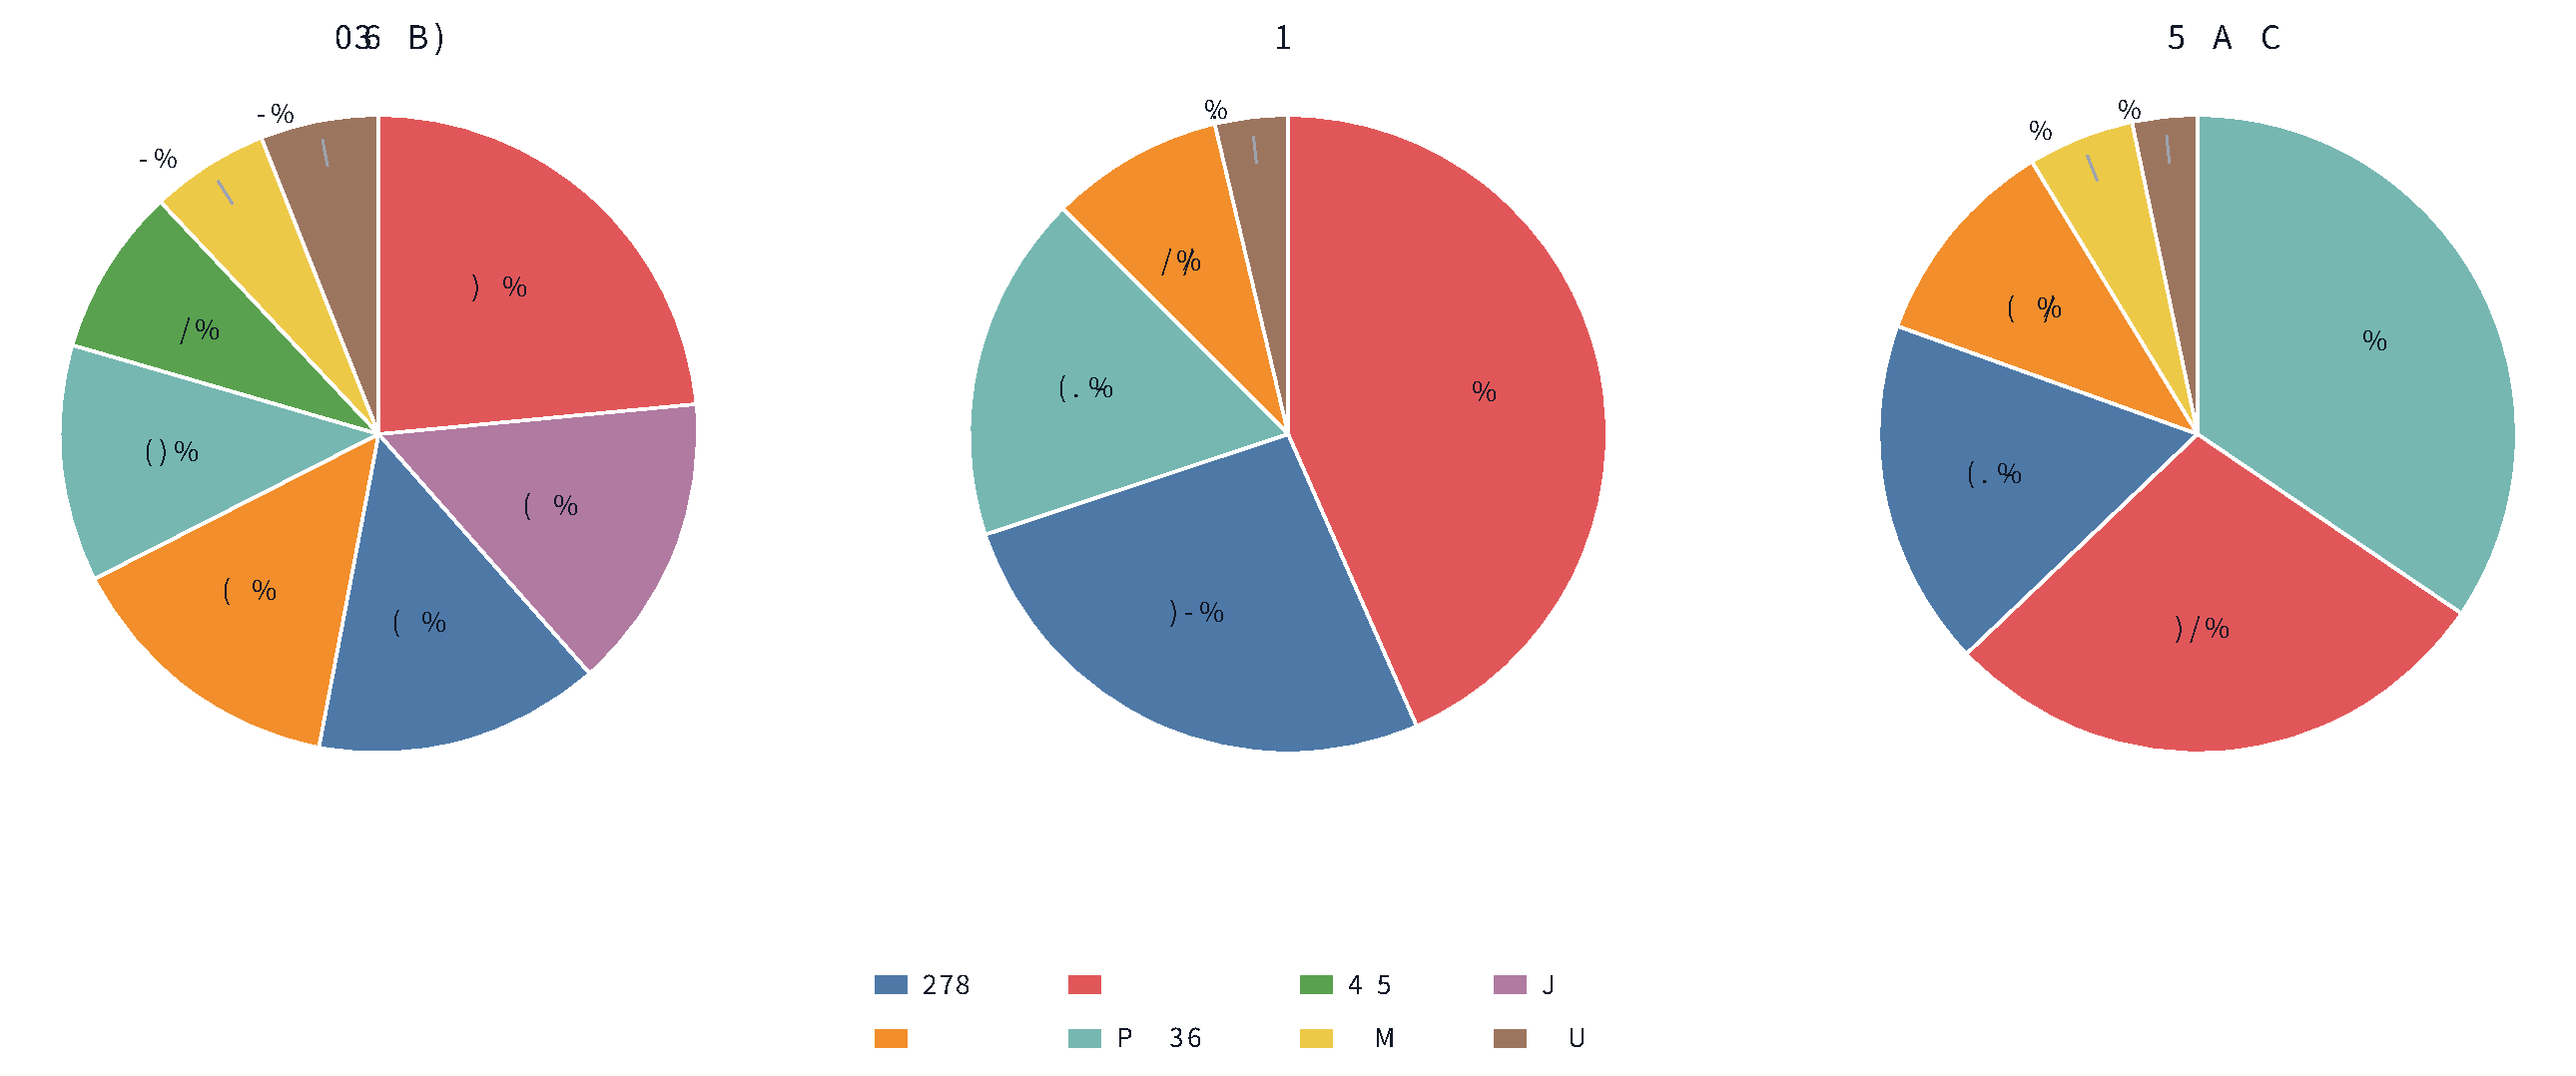
\includegraphics[width=\textwidth]{Figures-Src/Chap5-Experiment/fig5-1-fault-distribution/chart.pdf}
    \bicaption{\enspace 三个数据集的故障类型分布对比}{\enspace Fault Type Distribution Comparison Across Three Datasets}
    \label{fig:chap5_fault_distribution}
\end{figure}

\textbf{评估指标}：不同实验任务采用的评估指标有所区别。表\ref{tab:evaluation_framework}汇总了本文使用的指标及其对应任务。

\begin{table}[htbp]
    \centering
    \bicaption{\enspace 实验任务与评估指标对应关系}{\enspace Mapping Between Experimental Tasks and Evaluation Metrics}
    \label{tab:evaluation_framework}
    \ChapFiveTableSetup
    \begin{tabularx}{\textwidth}{>{\raggedright\arraybackslash}p{2.8cm}>{\raggedright\arraybackslash}X>{\raggedright\arraybackslash}p{4.5cm}}
        \toprule
        \rowcolor{\ChapFiveTableHeadColor}
        \textbf{实验任务} & \textbf{评估指标} & \textbf{说明} \\
        \midrule
        故障指纹检索 & Hit@1，Hit@3，Hit@5，MRR & 衡量相似故障能否稳定出现在排序前列 \\
        SOP 构建有效性 & 逃逸率，探索成功率，诊断成功率，任务完成率 & 衡量训练阶段的探索效果与测试阶段的执行结果 \\
        端到端根因定位性能 & Hit@1，Hit@3，Hit@5，MRR & 衡量真实根因在候选排序中的前部命中情况与整体排序质量 \\
        消融实验 & Hit@1，Hit@3，Hit@5，MRR & 比较移除不同机制后的性能变化 \\
        \bottomrule
    \end{tabularx}
\end{table}

其中，Hit@K 定义为：对于每个测试样本，若排序前 K 个候选中至少包含一个正确结果，则记为命中，否则记为未命中，最后对全部样本取平均。MRR 定义为首个正确结果排名倒数的平均值。

在端到端根因定位任务中，本文同样计算 Hit@3 和 Hit@5。这是因为各方法最终都会按照置信度返回候选根因列表，而在实际排障过程中，通常只保留前 5 个候选用于自动处置或人工复核。因此，Hit@5 既能反映真实根因是否进入“可操作候选窗口”，也能避免候选列表过长时削弱排序评估的实际意义。




%---------------------------------------------------------------------------%
%->> 5.3 故障指纹检索性能评估
%---------------------------------------------------------------------------%

\section{故障指纹检索性能评估}

本节评估传播感知多模态故障指纹构建方法 PMF 的检索效果。PMF 在整体框架中负责离线检索。它将历史故障转化为统一的故障指纹，用于召回相似案例，并为后续 SOP 绑定和在线诊断提供候选。本节关心的是，在“故障组件角色 + 故障类型”这一粒度下，PMF 能否把真正相似的历史故障稳定排到前列。

\begin{table}[htbp]
    \centering
    \bicaption{\enspace 数据集多模态异常占比统计}{\enspace Multi-Modal Anomaly Ratio Statistics of Datasets}
    \label{tab:anomaly_ratio}
    \ChapFiveTableSetup
    \setlength{\tabcolsep}{4pt}
    \resizebox{\textwidth}{!}{%
    \begin{tabular}{l|ccc|ccc|ccc}
        \toprule
        \rowcolor{\ChapFiveTableHeadColor}
        \textbf{模态} & \multicolumn{3}{c|}{\textbf{AIOps-25}} & \multicolumn{3}{c|}{\textbf{Bank}} & \multicolumn{3}{c}{\textbf{Market}} \\
        \rowcolor{\ChapFiveTableHeadColor}
        & \textbf{Metrics} & \textbf{Logs} & \textbf{Traces} & \textbf{Metrics} & \textbf{Logs} & \textbf{Traces} & \textbf{Metrics} & \textbf{Logs} & \textbf{Traces} \\
        \midrule
        异常占比 & 2.94\% & 3.79\% & 4.94\% & 3.12\% & 4.33\% & 4.87\% & 3.28\% & 2.07\% & 5.15\% \\
        \bottomrule
    \end{tabular}%
    }
    \setlength{\tabcolsep}{4.5pt}
    \ChapFiveTableNote{异常占比通过无监督异常检测方法计算。对于 Metrics 和 Traces 数据，采用 Isolation Forest 算法（contamination=5\%）识别偏离正常分布的异常数据点；对于 Logs 数据，统计 ERROR/WARN/FATAL 级别日志的占比。该统计基于每个数据集 30 个故障事件的采样分析。}
\end{table}

故障指纹检索实验在三个数据集上进行，设置如下。

\textbf{检索单元定义}：按照“故障组件角色 + 故障类型”对故障事件分组。只有当历史故障与查询故障在这两个维度上同时一致时，才视为相关样本。比如，\texttt{database-connection-pool + connection-exhaustion} 与 \texttt{database-connection-pool + slow-query} 虽然根因组件角色相同，但故障类型不同，因此属于不同检索目标；而发生在不同实例上的同角色数据库连接池耗尽事件，则归为同一组。

\textbf{训练/测试划分}：每个数据集按 60\%/40\% 划分训练集和测试集。训练集用于构建故障指纹库，测试集用于评估检索性能。为减小随机划分带来的波动，每组实验重复 5 次，结果取平均值。

\textbf{检索指标计算}：对于测试集中的每个故障事件，系统从故障指纹库中检索 Top-K 个最相似的历史案例。若 Top-K 候选中至少存在一个与查询故障在“组件角色 + 故障类型”上同时一致的案例，则该样本在 Hit@K 上记为命中。

\textbf{对比基线}：为便于与传统方法比较，本节选取六种基线：TF-IDF、MS-Rank、ART、DiagFusion、AnoFusion 和 BWGNN。TF-IDF 仅使用文本描述；MS-Rank 侧重多指标融合；ART 和 DiagFusion 分别代表注意力驱动的多模态建模和显式模态融合；AnoFusion 与 BWGNN 则代表图建模思路。对于只输出服务级得分、不能直接生成事件级向量的方法，本文依据其异常分布和排序结果构造对齐后的事件级表示，以支持统一检索评估。

表\ref{tab:fingerprint_recall}给出了不同方法在三个数据集上的检索结果，图\ref{fig:5-fingerprint-mrr-bar}展示了对应的 MRR。

\begin{table}[htbp]
    \centering
    \bicaption{\enspace 故障指纹检索性能对比}{\enspace Comparison of Fault Fingerprint Retrieval Performance}
    \label{tab:fingerprint_recall}
    \ChapFiveTableSetup
    \resizebox{\textwidth}{!}{%
    \begin{tabular}{l|ccc|ccc|ccc}
        \toprule
        \rowcolor{\ChapFiveTableHeadColor}
        \textbf{方法} & \multicolumn{3}{c|}{\textbf{AIOps-25}} & \multicolumn{3}{c|}{\textbf{Bank}} & \multicolumn{3}{c}{\textbf{Market}} \\
        \rowcolor{\ChapFiveTableHeadColor}
        & \textbf{Hit@1} & \textbf{Hit@3} & \textbf{Hit@5} & \textbf{Hit@1} & \textbf{Hit@3} & \textbf{Hit@5} & \textbf{Hit@1} & \textbf{Hit@3} & \textbf{Hit@5} \\
        \midrule
        TF-IDF & 23.74 & 41.75 & 54.00 & 22.40 & 38.93 & 51.05 & 19.89 & 36.06 & 48.49 \\
        MS-Rank & 26.88 & 44.63 & 56.88 & 25.03 & 41.93 & 52.93 & 22.92 & 39.10 & 50.52 \\
        BWGNN & 29.89 & 48.51 & 61.01 & 27.93 & 45.97 & 57.39 & 26.22 & 43.06 & 55.20 \\
        AnoFusion & 33.25 & 52.99 & 64.50 & 30.45 & 49.98 & 61.73 & 27.94 & 45.79 & 57.24 \\
        ART & 35.11 & 55.37 & 66.87 & 33.04 & 51.83 & 63.63 & 29.99 & 48.15 & 59.96 \\
        DiagFusion & 36.75 & 57.00 & 68.75 & 34.90 & 54.42 & 65.44 & 31.97 & 49.84 & 61.29 \\
        \midrule
        \textbf{PMF（本文方法）} & \textbf{53.26} & \textbf{72.01} & \textbf{81.37} & \textbf{49.95} & \textbf{68.36} & \textbf{79.02} & \textbf{46.79} & \textbf{64.95} & \textbf{75.38} \\
        \bottomrule
    \end{tabular}
    }
\end{table}

\begin{figure}[htbp]
    \centering
    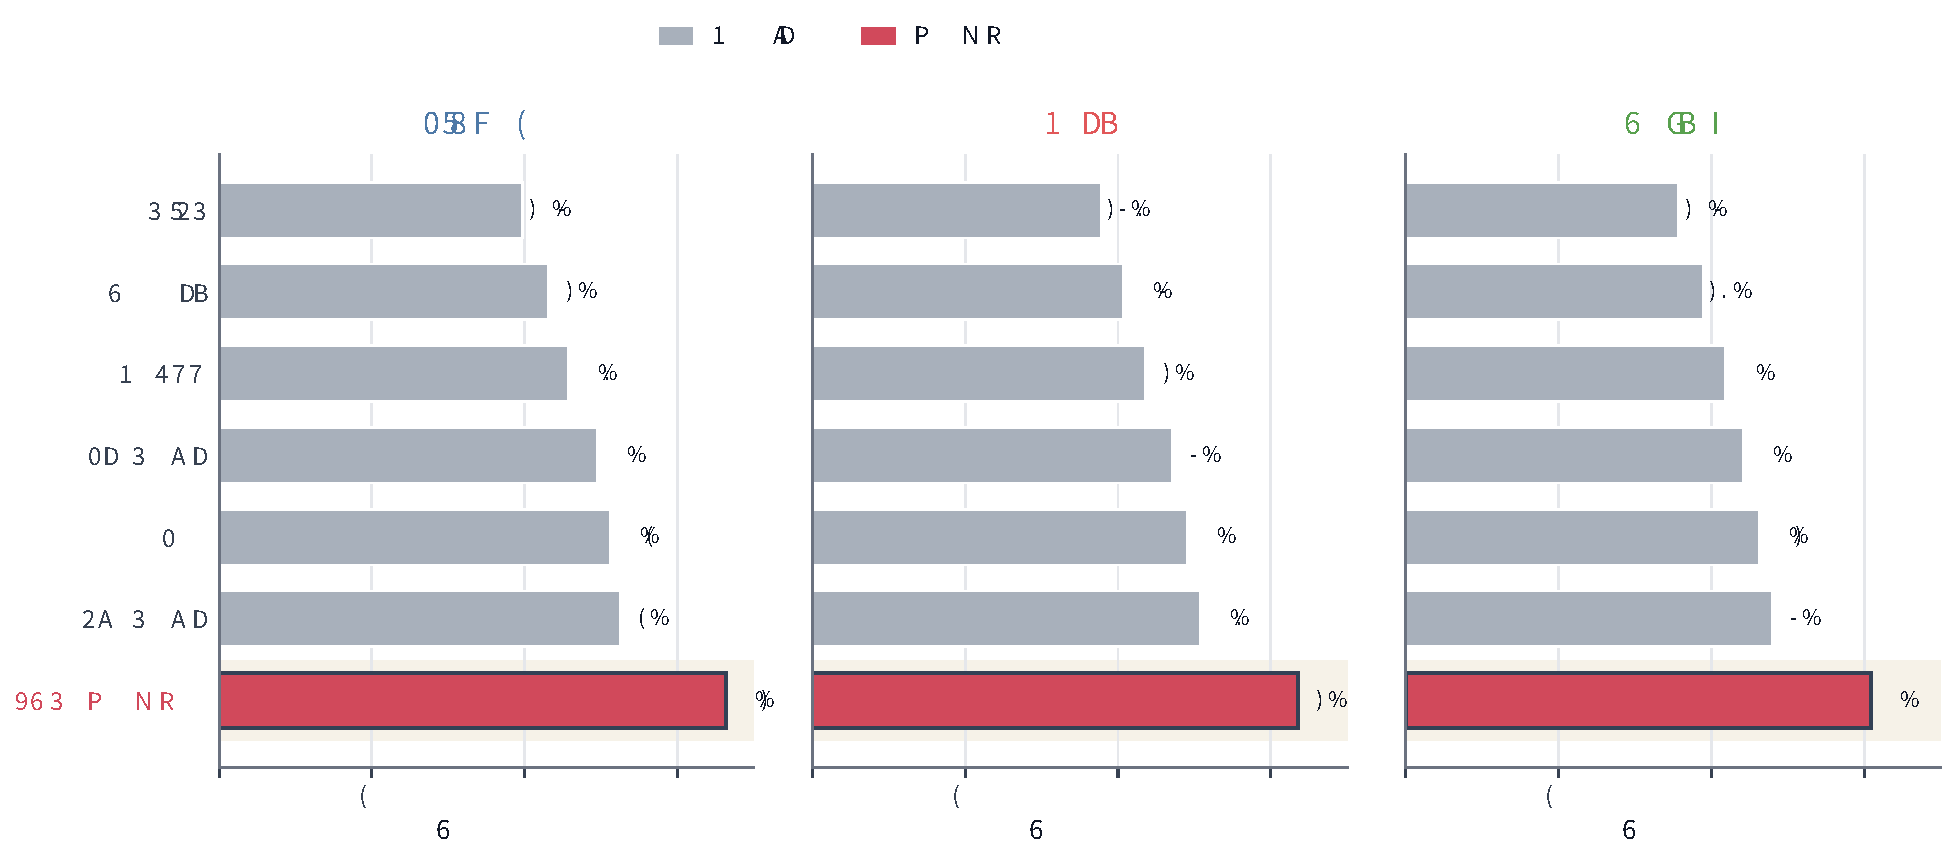
\includegraphics[width=\textwidth]{Figures-Src/Chap5-Experiment/fig5-2-fingerprint-mrr/chart.pdf}
    \bicaption{\enspace 故障指纹检索任务 MRR 对比}{\enspace MRR Comparison of Fault Fingerprint Retrieval}
    \label{fig:5-fingerprint-mrr-bar}
\end{figure}

从表\ref{tab:fingerprint_recall}和图\ref{fig:5-fingerprint-mrr-bar}可以看出，PMF 在三个数据集上的 Hit@1、Hit@3、Hit@5 和 MRR 均为最优。AIOps-25、Bank 和 Market 上的 Hit@1 分别达到 53.26\%、49.95\% 和 46.79\%，对应的 MRR 分别为 66.33\%、63.61\% 和 60.85\%。与各数据集上表现最好的传统基线 DiagFusion 相比，PMF 的 Hit@1 分别提高 16.51、15.05 和 14.82 个百分点，MRR 分别提高 13.83、12.82 和 12.91 个百分点。这表明，PMF 对“故障组件角色 + 故障类型”这一联合目标的刻画更准确，检索结果也更稳定。

从各基线的相对位置看，DiagFusion 整体最好，ART 次之，AnoFusion 随后，BWGNN 处于中间水平，MS-Rank 和 TF-IDF 较弱。这个结果并不意外。显式多模态融合、注意力建模和面向异常证据的融合策略，确实比单纯依赖文本相似度或多指标强度排序更适合微服务故障检索。不过，即便是表现最好的传统基线，与 PMF 之间仍有稳定差距。这说明，只依赖表层异常强度或单一模态对齐，还不足以区分“组件角色相同但故障类型不同”的案例。

结合 Hit@K 和 MRR 进一步看，PMF 的优势不仅体现在是否命中，还体现在正确案例出现得更靠前。以 AIOps-25 为例，PMF 的 Hit@3 为 72.01\%，比 DiagFusion 高 15.01 个百分点；在 Market 上，PMF 的 Hit@5 为 75.38\%，比 DiagFusion 高 14.09 个百分点。与此同时，MRR 的变化趋势与 Hit@1 基本一致，说明性能提升不是来自少量偶然命中，而是来自正确案例在排序前部的整体前移。换句话说，PMF 不只是“能找到”，而是“更早找到”。

这与 PMF 的表示方式有关。该方法不是简单拼接多模态异常信号，而是把传播路径、组件角色语义和跨模态证据放到同一个表示空间里处理。因此，面对“入口症状接近、内部成因不同”的故障时，PMF 更容易把真正相关的案例排到前面，把表面相似但根因不同的案例拉开。

从数据集本身看，AIOps-25 的整体结果最高，Bank 次之，Market 最低，这与三个数据集的服务规模和故障传播复杂度基本一致。尤其是在 Market 上，最强传统基线 DiagFusion 的 Hit@1 只有 31.97\%，MRR 为 47.94\%，说明在服务规模更大、传播链更长的场景下，局部异常和表面症状更容易混淆。即便如此，PMF 在 Market 上仍取得 46.79\% 的 Hit@1 和 60.85\% 的 MRR，说明它已经能够为后续的 SOP 绑定和在线诊断提供较为稳定的历史候选。

综合来看，PMF 在三个数据集上都表现出较好的检索稳定性和区分能力，能够在“故障组件角色 + 故障类型”这一粒度下有效召回相似历史故障。这个结果也为后续的 SOP 复用和在线诊断提供了可靠基础。

%---------------------------------------------------------------------------%
%->> 5.4 SOP自动化构建有效性评估
%---------------------------------------------------------------------------%

\section{SOP 自动化构建有效性评估}

本节评估 SOP 自动化构建方法的有效性。与关注最终排序结果的实验不同，这里更关注 SOP 是如何在迭代过程中逐步形成的：以故障指纹聚类簇为单位构建的 SOP，是否会在多轮增量更新中从一张空图逐步发展为可执行的诊断结构，并对簇内未见故障提供稳定支持。

在本文中，SOP 以“故障组件角色 + 故障类型”的故障指纹聚类簇为基本组织单元，也就是一个聚类簇对应一个 SOP。基于前文得到的 PMF 故障指纹，本文在三个数据集上完成聚类，并统计各数据集的聚类结果。表\ref{tab:sop_cluster_stats}给出了聚类簇数量及其规模分布。

\begin{table}[htbp]
    \centering
    \bicaption{\enspace SOP 构建实验的故障指纹聚类统计}{\enspace Fault Fingerprint Cluster Statistics for SOP Construction}
    \label{tab:sop_cluster_stats}
    \ChapFiveTableSetup
    \begin{tabular}{lccccc}
        \toprule
        \rowcolor{\ChapFiveTableHeadColor}
        \textbf{数据集} & \textbf{聚类簇数量} & \textbf{平均指纹数/簇} & \textbf{最小指纹数/簇} & \textbf{最大指纹数/簇} & \textbf{入选簇数量} \\
        \midrule
        AIOps-25 & 34 & 11.76 & 3 & 29 & 17 \\
        Bank & 16 & 8.50 & 2 & 16 & 8 \\
        Market & 20 & 7.40 & 2 & 14 & 10 \\
        \midrule
        \rowcolor{\ChapFiveTableStatColor}
        \textbf{合计/总体均值} & \textbf{70} & \textbf{9.77} & \textbf{2} & \textbf{29} & \textbf{35} \\
        \bottomrule
    \end{tabular}
\end{table}

实验从每个数据集中按簇规模降序选取前 50\% 的聚类簇，最终得到 35 个入选簇。这样做主要出于两点考虑：一是保证每个簇都有足够的历史样本支撑 SOP 的初始构建；二是尽量覆盖不同数据集中的高频故障模式，而不是把结论建立在单一数据集上。对于每个入选簇，本文都在簇内按 60\%/40\% 划分训练集和测试集。训练集用于从零构建并持续更新该簇对应的 SOP，测试集用于评估当前 SOP 对簇内未见故障的支持能力。

为避免歧义，本文将一个 Turn 定义为一次完整的“构建 + 评估”闭环。对每个入选簇，在第 $t$ 个 Turn 中，系统先利用第 $t-1$ 个 Turn 的 SOP 在训练集上执行离线构建，再使用更新后的 SOP 在测试集上执行评估。训练阶段中，针对簇内每个训练故障事件创建 10 个 \textit{Exploration Agent} 并行探索，收集 SOP 执行轨迹；随后对全部轨迹执行 1 次因果挖掘，提取决策单元并计算权重；最后由 \textit{RuleAgent} 更新当前 SOP。测试阶段中，针对簇内每个测试故障事件创建 4 个 \textit{Diagnosis Agent}，沿当前 SOP 执行诊断，并判断该事件是否被成功定位。整个实验连续执行 20 个 Turn。图\ref{fig:5-2-sop-metrics}中的结果，是三个数据集全部 35 个入选簇在各 Turn 上的平均值。

本节统计四类行为指标和两类结构指标。逃逸率定义为训练阶段触发逃逸的探索智能体占全部探索智能体的比例，用于反映当前 SOP 的覆盖不足程度；探索成功率定义为训练阶段成功定位根因的探索智能体占比，用于衡量当前 SOP 对历史样本的引导能力；诊断成功率定义为测试阶段成功定位根因的故障事件占测试事件总数的比例，用于衡量 SOP 对簇内未见实例的泛化能力；任务完成率定义为相关智能体成功调用 \texttt{conclude} 并输出结果的比例，用于衡量流程能否闭环，而不区分结论是否正确。SOP 节点数和边数记录的是该 Turn 经 \textit{RuleAgent} 更新后的图规模，因此若系统在某一 Turn 删除冗余节点、合并重复分支或重写条件边，这两个指标出现回落，反映的是结构整理，而不是知识退化。

图\ref{fig:5-2-sop-metrics}展示了 20 个 Turn 中的平均行为指标和结构变化。其中，图(a)给出逃逸率、探索成功率、诊断成功率和任务完成率，图(b)给出平均 SOP 节点数和边数的变化。

\begin{figure}[htbp]
    \centering
    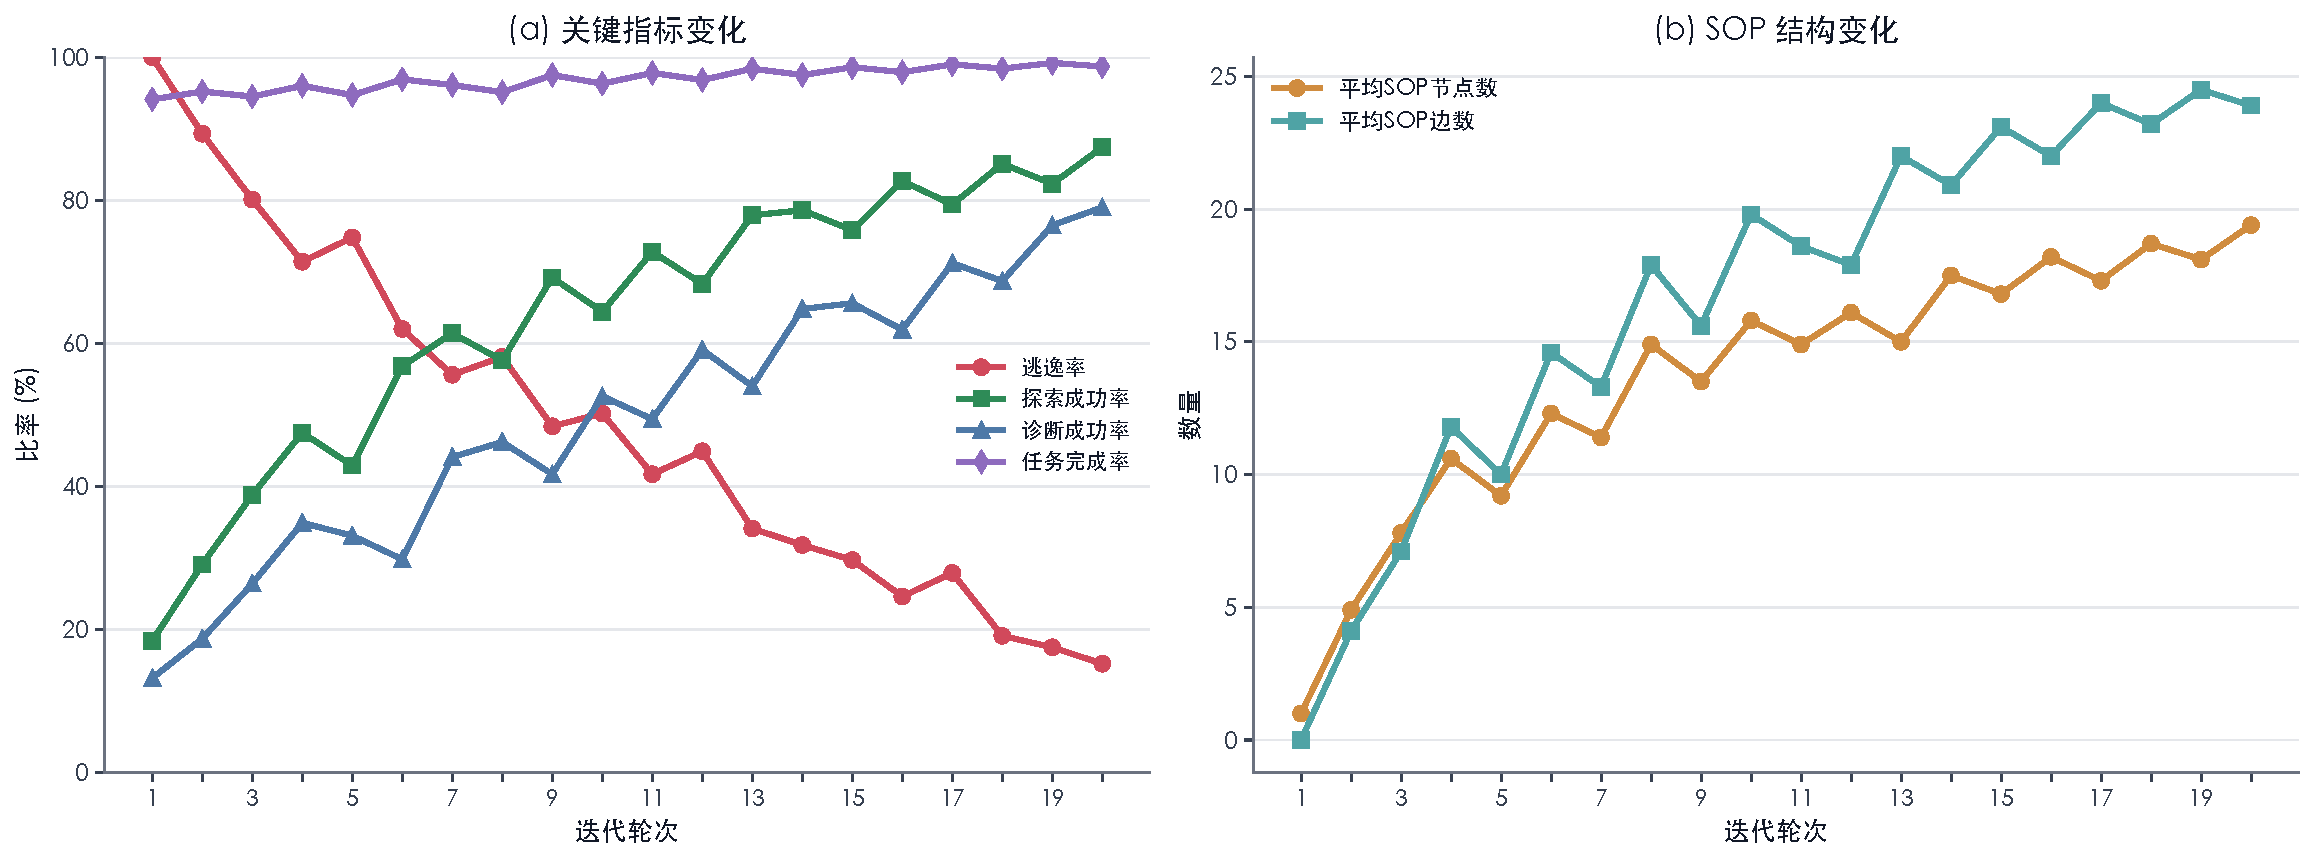
\includegraphics[width=\textwidth]{Figures-Src/Chap5-Experiment/fig5-4-sop-iteration-metrics/chart.pdf}
    \bicaption{\enspace 跨聚类簇平均的 SOP 构建迭代指标与结构变化}{\enspace Average Metric and Structure Evolution During SOP Construction Across Clusters}
    \label{fig:5-2-sop-metrics}
\end{figure}

从图\ref{fig:5-2-sop-metrics}可以看出，SOP 的形成并不是线性累加的过程，而是在“扩展—修剪—重组”中逐步收敛。整体趋势很清楚：逃逸率逐步下降，探索成功率和诊断成功率逐步上升，任务完成率始终保持在较高水平。但这些指标都不是单调变化的，尤其是中期阶段，结构调整和性能起伏交替出现。这一现象说明，SOP 的迭代不是简单堆叠路径，而是在不断补充主链、删去冗余、改写分支条件的过程中逐步收敛。

第 1 个 Turn 对应的是冷启动状态。此时每个聚类簇的初始 SOP 只有 1 个入口节点 \texttt{ROOT}，没有任何边，因此平均 SOP 节点数为 1.0，平均边数为 0.0，所有探索智能体都必须触发逃逸，逃逸率自然为 100\%。不过，首个 Turn 的任务完成率仍达到 94.1\%，说明即使缺少可用的 SOP 路径，大多数智能体仍然能够完成流程并输出结论。这一阶段的主要问题不在于流程无法完成，而在于结论质量仍然较弱：这一阶段的探索成功率和诊断成功率分别只有 18.6\% 和 13.8\%。

第 2 至 5 个 Turn 是主链快速成形阶段。平均 SOP 节点数从 4.9 增长到 10.6，随后在第 5 个 Turn 回落到 9.2；平均边数从 4.1 增长到 11.8，随后回落到 10.0。这说明系统在早期很快补出一条可用主链，但几轮之后就开始主动修剪。行为指标也呈现出对应变化：逃逸率从 89.3\% 下降到 71.4\%，随后在第 5 个 Turn 回升到 74.8\%；探索成功率从 29.1\% 提升到 47.5\%，随后回落到 42.9\%。这说明，早期阶段的主要收益并不来自图规模的持续扩大，而是来自主路径的快速形成以及后续的结构修整。

第 6 至 13 个 Turn 进入分支扩张和结构重写并行的阶段。此时节点数在 11.4 到 16.1 之间阶梯式上升，边数则在 13.3 到 22.0 之间波动得更明显。比如，从第 8 个 Turn 到第 9 个 Turn，平均节点数由 14.9 回落到 13.5，平均边数由 17.9 回落到 15.6；从第 11 个 Turn 到第 12 个 Turn，节点数从 14.9 增长到 16.1，但边数反而由 18.6 回落到 17.9；到第 13 个 Turn，边数又跃升到 22.0。这一阶段的图结构变化并不表现为节点数量的机械增长，而更多体现为连接关系的反复调整，以及新条件分支的逐步补充。

指标变化也表现出明显的先后次序。探索成功率通常比诊断成功率更早对结构变化作出反应。例如，第 6 个 Turn 时，探索成功率已经恢复到 56.8\%，但诊断成功率却回落到 29.8\%；之后探索成功率在第 8、10、12 个 Turn 出现局部回撤，诊断成功率则在第 9、11、13 个 Turn 出现更明显的滞后下跌。这个现象说明，结构调整首先会影响训练阶段的探索路径，而对未见样本的泛化效果往往要晚一拍才显现出来。也就是说，SOP 在训练阶段表现出的改进，并不意味着其在测试阶段的泛化能力会同步提升。

第 14 个 Turn 之后，系统进入后期稳定和长尾饱和阶段。此时平均 SOP 节点数基本稳定在 16.8 到 19.4 之间，只做小幅增删；平均边数仍在 20.9 到 24.5 之间持续调整，说明节点语义已经基本固定，但分支条件和连接关系还在细化。与此同时，逃逸率从 31.8\% 继续下降到 15.2\%，中间在第 17 个 Turn 短暂回升到 27.9\%；探索成功率在 78.6\% 到 87.4\% 之间震荡上升；诊断成功率则在 64.8\% 到 79.0\% 之间缓慢提升，且仍表现出一定滞后。逃逸率没有降到零，这一点反而是合理的：它说明高频诊断路径已经被较好覆盖，但系统仍为少量长尾故障保留了受控探索空间。与此同时，任务完成率在这一阶段始终维持在 97.5\% 到 99.2\% 之间，说明流程本身已经相当稳定。

另一个值得注意的现象是，任务完成率始终明显高于诊断成功率。到第 20 个 Turn，两者仍相差 19.7 个百分点。这说明 SOP 的“可执行”会先于“诊断准确”收敛。探索成功率与诊断成功率之间的差距也在逐步缩小：例如，第 13 个 Turn 两者相差 23.9 个百分点，而到第 20 个 Turn 收敛到 8.4 个百分点。这进一步说明，结构改写带来的收益通常先在训练侧显现，随后才逐步传递到簇内未见样本上。

下面以 AIOps-25 数据集中“数据库连接池耗尽”聚类簇为例，说明 SOP 自动化构建过程中的中间产出。

\textbf{SOP 执行轨迹生成}。针对该故障簇中的一次故障事件，系统创建 10 个探索智能体并行探索，其中 6 条轨迹成功定位根因，4 条轨迹由于分支选择偏离而失败。成功轨迹通常呈现出相似的主证据链：先从入口服务的请求延迟异常出发，沿调用链追踪到数据库访问路径，再结合连接等待时间、活跃连接数和连接池配置完成定位。失败轨迹则更多停留在上游业务服务或缓存侧症状，没有及时沿传播链继续向下游收敛。

\textbf{决策单元提取与权重计算}。系统将这 10 条轨迹拆分为 37 个原始决策单元，经过语义对齐和 DBSCAN 聚类后得到 9 个语义簇。例如，“检查 DB 连接池状态”“查看数据库活跃连接数”和“分析连接池占用率”被归并为同一语义簇，并统一表示为 \texttt{CHECK\_DB\_CONN\_POOL}。在该案例中，得分最高的三个决策单元分别是“检查请求延迟分布”（0.91）、“追踪数据库连接等待”（0.88）和“分析连接池配置”（0.84），说明这三步对根因收敛的贡献最稳定。

\textbf{规则智能体组织}。规则智能体根据带权决策单元将主链和分支组织成 SOP 图。初始主链包含 7 个节点和 6 条边，对应“入口服务时延异常 $\rightarrow$ 下游数据库访问异常 $\rightarrow$ 连接池状态检查 $\rightarrow$ 根因确认”的核心路径。随后在回放验证时，系统发现“连接池占用未满但连接等待显著升高”的场景没有被主链覆盖，于是补充了通向“检查慢查询”和“检查长事务”的条件分支。经过 3 轮修正后，最终 SOP 稳定为 8 个节点和 7 条边。

这个案例说明，SOP 自动化构建并不是简单保留某一条成功轨迹，而是从同一故障指纹聚类簇内的成功轨迹和失败轨迹中，提取那些能够反复帮助诊断收敛的局部决策，再把它们组织成可执行的图结构。这样得到的 SOP 更适合在簇内后续故障中复用，也更符合在线诊断阶段“先沿已有经验推进，必要时再受控探索”的执行方式。

综合来看，SOP 自动化构建方法能够在多轮迭代中逐步形成较稳定的可执行结构。其演化过程不是线性的，而是伴随着主链搭建、分支扩张和结构整理交替进行。随着迭代推进，SOP 对高频故障路径的覆盖不断提高，对簇内未见故障的支持能力也逐步增强，这说明该方法具备持续积累和稳定复用诊断经验的能力。

%---------------------------------------------------------------------------%
%->> 5.5 端到端诊断性能评估
%---------------------------------------------------------------------------%

\section{端到端诊断性能评估}

本节在相同的数据划分设置下比较传统基线、大语言模型基线与本文方法的端到端根因定位性能，重点观察不同方法在真实故障场景中的排序差异。

本文方法由三个关键部分组成：PMF 历史案例检索、SOP 引导执行以及 SOP 未覆盖时的逃逸机制，并在在线阶段额外引入焦点与感知域约束以减少无关证据干扰。

端到端诊断性能评估在三个数据集上进行。对每个数据集，都采用 70\%/30\% 的训练/测试划分比例。训练集用于构建故障指纹库和 SOP，测试集用于端到端性能评估。为减小随机划分带来的波动，每组实验重复 3 次并取平均值。

\textbf{传统基线}：为保持与第5.3节的一致性，传统方法沿用同一组六种基线：TF-IDF、MS-Rank、ART、DiagFusion、AnoFusion 和 BWGNN。这样可以同时观察这些方法在“离线相似案例检索”和“在线根因定位排序”两个任务中的相对表现。

\textbf{大语言模型基线}：本节进一步对比 ReAct~\cite{yao2022react}、RCAgent~\cite{wang2024rcagent}、mABC~\cite{zhang2024mabc}、OpenRCA（其论文中的 RCA-agent 基线）~\cite{xu2025openrca} 和 Flow-of-Action~\cite{pei2025flowofaction}。其中，Flow-of-Action 采用固定的 SOP/动作流模板执行诊断，属于知识增强的大语言模型方法，不属于传统统计方法。为保证公平性，上述大语言模型方法均统一采用 MiniMax M2.1 作为底层模型。

评估指标采用 Hit@1、Hit@3、Hit@5 和 MRR。这里的“命中”指真实根因组件是否出现在前 K 个候选中。之所以特别统计 Hit@5，是因为本文与各大语言模型基线在输出阶段都统一返回按置信度排序的 Top-5 根因候选，超过 5 个候选会显著增加人工复核成本，并削弱候选排序在真实运维中的可执行性。

表\ref{tab:e2e_comparison}展示了不同方法在三个数据集上的端到端根因定位性能，图\ref{fig:5-e2e-mrr-bar}给出了对应的 MRR 结果。

\begin{table}[htbp]
    \centering
    \bicaption{\enspace 端到端诊断性能对比}{\enspace End-to-End Diagnosis Performance Comparison}
    \label{tab:e2e_comparison}
    \ChapFiveTableSetup
    \setlength{\tabcolsep}{2.8pt}
    \resizebox{\textwidth}{!}{%
    \begin{tabular}{cl|ccc|ccc|ccc}
        \toprule
        \rowcolor{\ChapFiveTableHeadColor}
        \textbf{类型} & \textbf{方法} & \multicolumn{3}{c|}{\textbf{AIOps-25}} & \multicolumn{3}{c|}{\textbf{Bank}} & \multicolumn{3}{c}{\textbf{Market}} \\
        \rowcolor{\ChapFiveTableHeadColor}
        & & \textbf{Hit@1} & \textbf{Hit@3} & \textbf{Hit@5} & \textbf{Hit@1} & \textbf{Hit@3} & \textbf{Hit@5} & \textbf{Hit@1} & \textbf{Hit@3} & \textbf{Hit@5} \\
        \midrule
        \multirow{6}{*}{传统} & TF-IDF & 7.76 & 18.31 & 29.99 & 6.59 & 15.63 & 27.09 & 5.27 & 14.26 & 24.78 \\
        & MS-Rank & 8.89 & 20.02 & 32.27 & 8.17 & 17.13 & 29.45 & 6.77 & 15.74 & 26.26 \\
        & BWGNN & 11.67 & 24.17 & 36.14 & 9.84 & 22.15 & 33.62 & 8.27 & 19.56 & 30.84 \\
        & AnoFusion & 12.50 & 26.12 & 38.60 & 11.44 & 23.72 & 35.24 & 9.80 & 21.08 & 32.34 \\
        & ART & 13.33 & 29.18 & 40.29 & 12.26 & 25.37 & 36.02 & 10.57 & 21.89 & 33.92 \\
        & DiagFusion & 14.44 & 30.00 & 42.49 & 13.07 & 27.05 & 38.54 & 12.02 & 24.06 & 35.29 \\
        \midrule
        \multirow{5}{*}{大语言模型} & OpenRCA (RCA-agent) & 18.06 & 37.77 & 53.33 & 16.40 & 35.26 & 49.98 & 14.26 & 30.89 & 45.93 \\
        & ReAct & 18.88 & 39.17 & 54.45 & 17.20 & 36.06 & 50.85 & 15.05 & 31.62 & 46.62 \\
        & RCAgent & 31.42 & 53.06 & 66.96 & 27.89 & 49.21 & 61.46 & 24.87 & 45.15 & 58.64 \\
        & mABC & 40.84 & 63.04 & 76.65 & 37.70 & 59.02 & 72.97 & 35.37 & 54.90 & 69.23 \\
        & Flow-of-Action & 46.11 & 67.49 & 79.72 & 41.85 & 62.28 & 75.41 & 39.11 & 57.15 & 71.43 \\
        \midrule
        & \textbf{本文方法} & \textbf{58.03} & \textbf{79.18} & \textbf{88.35} & \textbf{54.15} & \textbf{75.41} & \textbf{86.04} & \textbf{49.61} & \textbf{70.59} & \textbf{81.89} \\
        \bottomrule
    \end{tabular}
    }
    \setlength{\tabcolsep}{4.5pt}
\end{table}

\begin{figure}[htbp]
    \centering
    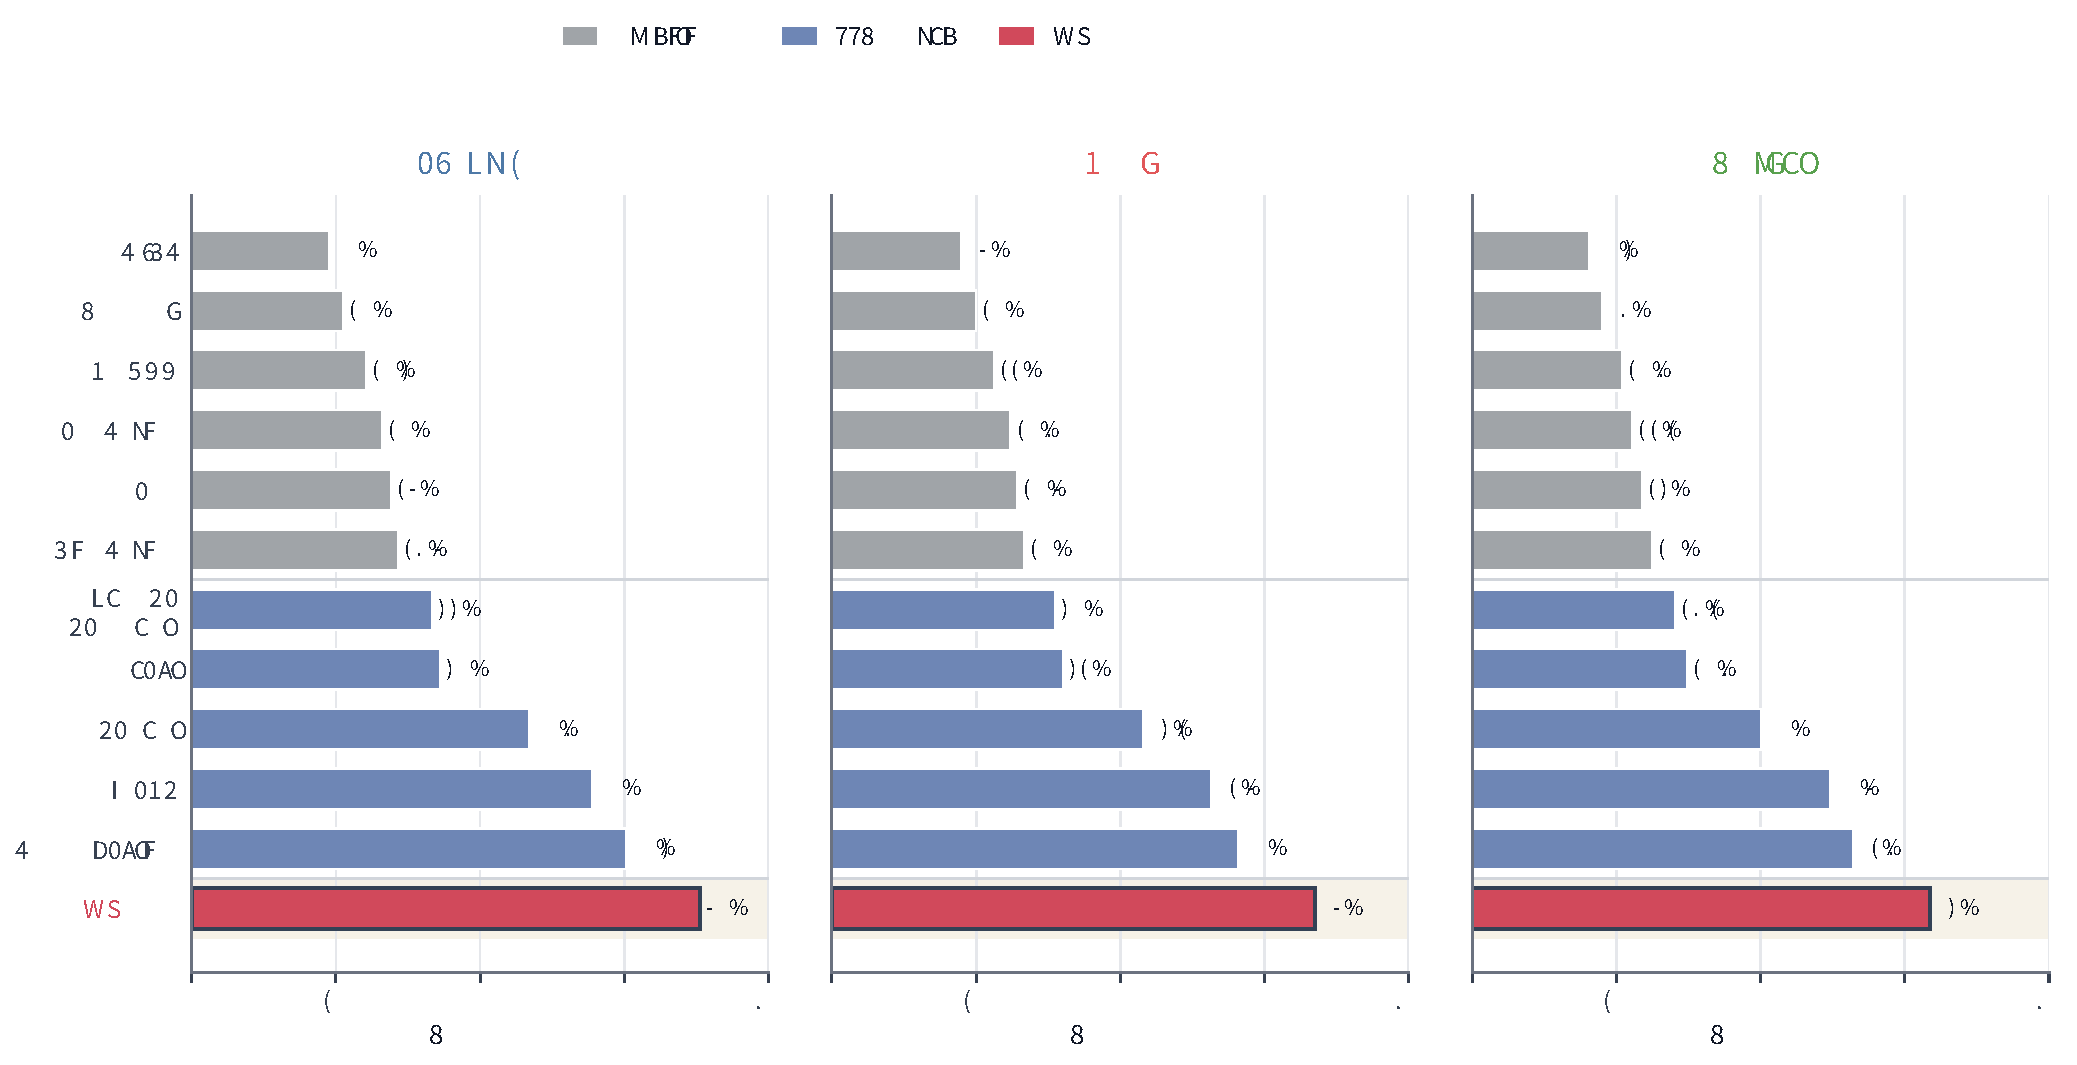
\includegraphics[width=\textwidth]{Figures-Src/Chap5-Experiment/fig5-5-e2e-mrr/chart.pdf}
    \bicaption{\enspace 端到端诊断任务 MRR 对比}{\enspace MRR Comparison of End-to-End Diagnosis}
    \label{fig:5-e2e-mrr-bar}
\end{figure}

表\ref{tab:e2e_comparison}和图\ref{fig:5-e2e-mrr-bar}表明，本文方法在三个数据集上的 Hit@1、Hit@3、Hit@5 和 MRR 均为最佳。其在 AIOps-25、Bank 和 Market 上的 Hit@1 分别达到 58.03\%、54.15\% 和 49.61\%，对应的 MRR 分别达到 70.49\%、66.99\% 和 63.53\%。与最强大语言模型基线 Flow-of-Action 相比，本文方法的 Hit@1 分别提升 11.92、12.30 和 10.50 个百分点，MRR 分别提升 10.16、10.61 和 10.71 个百分点，这说明，本文方法不仅提高了首位命中率，也能在统一限制为 Top-5 的候选列表中更稳定地将真实根因排到前部。

从整体层次看，传统方法在端到端任务上的表现显著弱于主流大语言模型方法。最强传统基线 DiagFusion 在三个数据集上的 Hit@1 也仅为 14.44\%、13.07\% 和 12.02\%，MRR 分别为 28.66\%、26.64\% 和 24.94\%。在传统方法内部，DiagFusion 整体最强，ART 和 AnoFusion 处于较高水平，BWGNN 居中，而 TF-IDF 与 MS-Rank 明显更弱。这说明传统统计或图建模方法确实能够压缩可疑范围，但它们主要依赖离线异常关联和静态排序，尚不足以支撑微服务故障诊断所需要的多轮证据收集、路径切换和上下文更新。

大语言模型基线则呈现出更符合任务难度的层次结构。OpenRCA（RCA-agent）与 ReAct 的 Hit@1 只比最强传统方法略高，例如在 AIOps-25 上分别仅高出 3.62 和 4.44 个百分点，在 Bank 上高出 3.33 和 4.13 个百分点，在 Market 上高出 2.24 和 3.03 个百分点，说明单纯依赖通用工具调用和 ReAct 式交互策略，只能带来有限增益；RCAgent 在 AIOps-25 上已达到 31.42\% 的 Hit@1，mABC 和 Flow-of-Action 则进一步进入 40\% 以上区间。在更难的 Bank 与 Market 上，虽然整体数值有所回落，但 OpenRCA（RCA-agent）/ReAct、RCAgent、mABC、Flow-of-Action 之间的层次关系仍保持稳定，说明引入更强的流程约束和更系统的经验利用，确实能够持续改善端到端排序质量。

本文方法对传统方法和大语言模型基线都保持了明显优势。以 AIOps-25 为例，本文方法的 Hit@1 为 58.03\%，比最强传统基线 DiagFusion 高 43.59 个百分点，MRR 高 41.83 个百分点；在 Bank 上分别高 41.08 和 40.35 个百分点；在 Market 上也仍高出 37.59 和 38.59 个百分点。更重要的是，本文方法相对 Flow-of-Action 的差异不应只理解为单次定位指标更高。指标提升只是表层表现，真正的核心差异在于本文方法形成了“历史案例检索 - SOP 自动化构建 - 在线执行 - 结果回流更新”的闭环流程，而 Flow-of-Action 本质上仍是静态模板驱动的在线执行方法。

Flow-of-Action 工作提出的固定动作流模板能够显著压缩自主探索空间，因此相比 OpenRCA（RCA-agent）、ReAct、RCAgent 和 mABC 更容易保持稳定排序；但它仍然依赖预定义模板，既不能从历史诊断轨迹中自动构建 SOP，也无法把在线新经验稳定回流到知识库中。本文方法则先由 PMF 缩小候选历史案例范围，再由自动构建且可持续更新的角色化 SOP 约束运行路径，最后用逃逸机制补足 SOP 尚未覆盖的分支。因此，本文方法相对 Flow-of-Action 的最大优势并不只是更高的 Hit@1 或 MRR，而是具备持续沉淀和扩展诊断知识的闭环能力。

这种差异在复杂场景下更明显。Market 仍然是最难的端到端数据集，无论传统方法还是大语言模型方法，其 Hit@1 与 MRR 都普遍低于 AIOps-25 和 Bank；即便如此，本文方法在 Market 上仍保持了 49.61\% 的 Hit@1 和 63.53\% 的 MRR，明显高于 Flow-of-Action 的 39.11\% 和 52.82\%。这说明，在复杂拓扑下，仅依赖统计排序或静态动作模板都不足以支撑稳定诊断，历史经验检索、动态 SOP 约束和闭环更新需要结合起来考虑。

%---------------------------------------------------------------------------%
%->> 5.6 消融实验
%---------------------------------------------------------------------------%

\section{消融实验}

本节通过消融实验分析 SOP 引导、逃逸机制以及焦点与感知域约束对端到端根因定位性能的影响。实验在 AIOps-25 数据集上进行。该数据集样本规模较大，故障类型也较丰富，更适合观察不同机制对排序前部质量的影响。

为分别考察三类机制的作用，本文构造了以下三个变体。

\textbf{w/o SOP 引导}：移除 SOP 提供的运行时经验指导，诊断智能体改为采用纯 ReAct 风格的自主探索。该变体用于检验结构化经验约束是否构成了性能提升的主要来源。

\textbf{w/o 逃逸机制}：移除逃逸机制。当当前 SOP 无法覆盖故障场景时，诊断智能体只能沿现有路径继续尝试，无法扩展新的分支。该变体用于考察受控探索对未知或半未知故障的作用。

\textbf{w/o 焦点与感知域约束}：移除焦点与感知域约束，诊断智能体可以在全局范围内自由收集证据。该变体用于分析局部化观测约束在抑制噪声方面的贡献。

表\ref{tab:ablation}给出了各消融变体在 AIOps-25 数据集上的结果。

\begin{table}[htbp]
    \centering
    \bicaption{\enspace 消融实验结果（AIOps-25 数据集）}{\enspace Ablation Study Results on AIOps-25}
    \label{tab:ablation}
    \ChapFiveTableSetup
    \begin{tabular}{lcccc}
        \toprule
        \rowcolor{\ChapFiveTableHeadColor}
        \textbf{方法变体} & \textbf{Hit@1(\%)} & \textbf{Hit@3(\%)} & \textbf{Hit@5(\%)} & \textbf{MRR(\%)} \\
        \midrule
        \textbf{本文方法} & \textbf{58.04} & \textbf{79.45} & \textbf{88.05} & \textbf{70.78} \\
        w/o SOP 引导 & 19.19 & 39.46 & 54.46 & 34.57 \\
        w/o 逃逸机制 & 43.05 & 64.43 & 77.75 & 57.60 \\
        w/o 焦点与感知域约束 & 50.01 & 71.12 & 81.94 & 63.32 \\
        \bottomrule
    \end{tabular}
\end{table}

从表\ref{tab:ablation}可以看出，三类机制都会影响最终排序质量，而且影响程度存在明显差异。其中，SOP 引导的作用最为关键。移除 SOP 引导后，Hit@1 从 58.04\% 降至 19.19\%，MRR 从 70.78\% 降至 34.57\%，分别下降 38.85 和 36.21 个百分点，降幅明显大于另外两项消融。更重要的是，这一变体的表现已经接近 ReAct 和 OpenRCA 这类通用大语言模型智能体。这说明，一旦失去 SOP 提供的结构化经验约束，诊断过程虽然仍然可以调用工具并持续推理，但整体行为已经退化为通用的搜索式诊断。也就是说，本文方法的优势并不只是多了一层流程模板，而在于具备了可自动构建、可持续更新的 SOP 体系。

移除逃逸机制后，性能下降幅度次之。Hit@1、Hit@3、Hit@5 和 MRR 分别下降 14.99、15.02、10.30 和 13.18 个百分点。这表明，当现有 SOP 还不能完全覆盖真实故障场景时，保留结构外的受控探索是必要的。如果智能体只能在已有路径上反复尝试，那么一旦当前故障落在 SOP 的覆盖边界之外，诊断过程就很容易在错误分支附近过早收敛。

移除焦点与感知域约束后，性能也出现了稳定下降，但降幅相对较小。Hit@1、Hit@3、Hit@5 和 MRR 分别下降 8.03、8.33、6.11 和 7.46 个百分点。这个结果说明，该机制的主要作用不是提供新的诊断路径，而是在既有路径上减少无关证据的干扰，降低大语言模型被全局异常误导的概率。换句话说，焦点与感知域约束更像是一层局部化的证据过滤机制，它提升的是推理稳定性，而不是直接增加搜索能力。

综合来看，三类机制的作用分工是清楚的。SOP 引导决定了诊断过程是否能够沿着已有经验有序展开；逃逸机制负责在 SOP 覆盖不足时补出新的路径，避免系统困在错误分支中；焦点与感知域约束则用于压缩无关证据，减少噪声对排序结果的影响。三者共同作用，才形成了前述端到端实验中的高位性能表现，也支撑了本文“经验检索—SOP 执行—结果回流更新”的闭环诊断框架。

%---------------------------------------------------------------------------%
%->> 本章小结
%---------------------------------------------------------------------------%

\section{本章小结}

本章从故障指纹检索、SOP 自动化构建、端到端根因定位和消融实验四个方面，对本文方法进行了系统评估。

实验结果表明，PMF 在三个公开数据集上的故障指纹检索性能均优于对比基线，说明传播感知多模态故障指纹能够在“故障组件角色 + 故障类型”这一粒度上稳定召回相似历史案例。SOP 自动化构建实验进一步表明，以故障指纹聚类簇为单位进行增量更新是可行的。随着迭代推进，SOP 结构经历了主链形成、分支扩展和后期整理的过程：系统从只有 1 个节点、0 条边和 100\% 逃逸率的初始状态出发，最终将平均逃逸率降至 15.2\%，将诊断成功率提升至 79.0\%，同时任务完成率始终保持在 94\% 以上。这说明自动构建得到的 SOP 具有较好的可执行性，也能够对簇内未见故障提供稳定支持。

端到端根因定位实验显示，本文方法在三个数据集上的 Hit@1、Hit@3、Hit@5 和 MRR 均为最佳。与最强的大语言模型基线 Flow-of-Action 相比，本文方法的 Hit@1 仍保持了 10.50 到 12.30 个百分点的稳定优势。消融实验进一步说明，SOP 引导、逃逸机制和焦点与感知域约束都会影响最终性能，其中 SOP 引导贡献最大；移除该机制后，系统性能会明显回落到通用大语言模型智能体附近。逃逸机制次之，主要用于处理 SOP 尚未覆盖的故障场景；焦点与感知域约束则主要提升推理过程的稳定性。

总体来看，本章实验验证了本文方法的优势不仅体现在更高的根因定位准确率上，也体现在方法结构本身。通过将历史案例检索、SOP 自动构建、在线执行和结果回流更新连接起来，本文形成了一个能够持续积累和复用诊断经验的闭环框架。
